\section{Vectores Aleatorios. Parte 2}

\begin{ejercicio}
    Sea la función de densidad del vector $(X,Y)$ dada por:
    \begin{equation*}
        f(x, y) = \begin{cases}
            k\left[\dfrac{xy}{2}+1\right] & 0<x<1,~-1<y<1, \\
            0 & \text{en otro caso}.
        \end{cases}
    \end{equation*}
    Se considera la transformación $Z=X-Y$, $T=X+2Y$. Hallar la función de densidad de probabilidad conjunta de la variable transformada $(Z,T)$.\\

    Buscamos en primer lugar el valor de $k$:
    \begin{align*}
        1&=\int_{-\infty}^{+\infty} \int_{-\infty}^{+\infty} f(x, y) \, dx \, dy = \int_{0}^{1} \int_{-1}^{1} k\left[\dfrac{xy}{2}+1\right] \, dy \, dx
        =\\&= k\int_{0}^{1} \left[\dfrac{xy^2}{4}+y\right]_{-1}^{1} \, dx = k\int_{0}^{1} \left[\dfrac{x}{4}+1-\dfrac{x}{4}+1\right] \, dx
        =\\&= k\int_{0}^{1} 2 \, dx = k\left[2x\right]_0^1 = 2k \Longrightarrow k=\frac{1}{2}
    \end{align*}

    Definimos ahora la función:
    \Func{g}{\bb{R}^2}{\bb{R}^2}{(X,Y)}{(Z,T)=(X-Y,X+2Y)}

    Para obtener $g^{-1}$, buscamos obtener $X,Y$ en función de $Z,T$:
    \begin{equation*}
        \left\{\begin{aligned}
            Z&=X-Y, \\
            T&=X+2Y.
        \end{aligned}\right\}\Longrightarrow
        Z-T=-3Y\Longrightarrow Y=\dfrac{T-Z}{3}\Longrightarrow X=\dfrac{2Z+T}{3}.
    \end{equation*}

    Por tanto, tenemos que:
    \Func{g^{-1}}{\bb{R}^2}{\bb{R}^2}{(Z,T)}{(X,Y)=\left(\dfrac{2Z+T}{3},\dfrac{T-Z}{3}\right)}

    Tenemos que todas las componentes de $g^{-1}$ son derivables:
    \begin{align*}
        \dfrac{\partial X}{\partial Z}(T,Z)&=\nicefrac{2}{3}, & \dfrac{\partial X}{\partial T}(Z,T)&=\nicefrac{1}{3},\\
        \dfrac{\partial Y}{\partial Z}(Z,T)&=\nicefrac{-1}{3}, & \dfrac{\partial Y}{\partial T}(Z,T)&=\nicefrac{1}{3}.
    \end{align*}

    Además, tenemos que:
    \begin{equation*}
        \det Jg^{-1}(z,t)=\begin{vmatrix}
            \nicefrac{2}{3} & \nicefrac{1}{3} \\
            \nicefrac{-1}{3} & \nicefrac{1}{3}
        \end{vmatrix}=\frac{1}{3^2}\begin{vmatrix}
            2 & 1 \\
            -1 & 1
        \end{vmatrix}=\frac{1}{3^2}(2-(-1))=\frac{3}{3^2}=\frac{1}{3}\neq 0 \qquad \forall (z,t)\in\bb{R}^2.
    \end{equation*}

    Por tanto, $(Z,T)=g(X,Y)$ es un vector aleatorio continuo. Buscamos ahora la función de densidad de probabilidad de $(Z,T)$:
    \begin{align*}
        &f_{(Z,T)}(z, t)=f_{(X,Y)}\left(\dfrac{2z+t}{3},\dfrac{t-z}{3}\right)\cdot \left|\det Jg^{-1}\left(z,t\right)\right|
        =\\&= \begin{cases}
            \dfrac{1}{3}\cdot \dfrac{1}{2}\left[\dfrac{\frac{2z+t}{3}\cdot \frac{t-z}{3}}{2}+1\right]
            =\dfrac{1}{6}\left[\dfrac{(2z+t)(t-z)}{18}+1\right] & 0<\dfrac{2z+t}{3}<1,~-1<\dfrac{t-z}{3}<1, \\
            0 & \text{en otro caso}.
        \end{cases}
    \end{align*}

    Por tanto, la función de densidad de probabilidad de $(Z,T)$ es:
    \begin{equation*}
        f_{(Z,T)}(z, t) = \begin{cases}
            \dfrac{1}{6}\left[\dfrac{(2z+t)(t-z)}{18}+1\right] & 0<2z+t<3,~-3<t-z<3, \\
            0 & \text{en otro caso}.
        \end{cases}
    \end{equation*}
\end{ejercicio}

\begin{ejercicio}
    Sea $(X,Y)$ un vector aleatorio bidimensional con función de densidad de probabilidad
    \begin{equation*}
        f(x, y) = \begin{cases}
            \exp(-x-y) & x>0,~y>0, \\
            0 & \text{en otro caso}.
        \end{cases}
    \end{equation*}
    Calcular la función de densidad de probabilidad de la variable aleatoria $Z=X+2Y$, a partir del cálculo de la densidad de probabilidad conjunta de la variable aleatoria bidimensional transformada $(Z,T)$, siendo $Z=X+2Y$, y $T=Y$.

    Definimos la transformación:
    \Func{g}{\bb{R}^2}{\bb{R}^2}{(X,Y)}{(Z,T)=(X+2Y,Y)}

    Para obtener $g^{-1}$, buscamos obtener $X,Y$ en función de $Z,T$:
    \begin{equation*}
        \left\{\begin{aligned}
            Z&=X+2Y, \\
            T&=Y.
        \end{aligned}\right\}\Longrightarrow
        \left\{\begin{aligned}
            X&=Z-2T, \\
            Y&=T.
        \end{aligned}\right.
    \end{equation*}

    Por tanto, tenemos que:
    \Func{g^{-1}}{\bb{R}^2}{\bb{R}^2}{(Z,T)}{(X,Y)=(Z-2T,T)}

    Tenemos que todas las componentes de $g^{-1}$ son derivables:
    \begin{align*}
        \dfrac{\partial X}{\partial Z}(Z,T)&=1, & \dfrac{\partial X}{\partial T}(Z,T)&=-2,\\
        \dfrac{\partial Y}{\partial Z}(Z,T)&=0, & \dfrac{\partial Y}{\partial T}(Z,T)&=1.
    \end{align*}

    Además, tenemos que:
    \begin{equation*}
        \det Jg^{-1}(z,t)=\begin{vmatrix}
            1 & -2 \\
            0 & 1
        \end{vmatrix}=1\neq 0 \qquad \forall (z,t)\in\bb{R}^2.
    \end{equation*}

    Por tanto, $(Z,T)=g(X,Y)$ es un vector aleatorio continuo. Buscamos ahora la función de densidad de probabilidad de $(Z,T)$:
    \begin{align*}
        &f_{(Z,T)}(z, t)=f_{(X,Y)}(z-2t,t)\cdot \left|\det Jg^{-1}(z,t)\right|
        =\\&= \begin{cases}
            \exp(-(z-2t)-t)=\exp(-z+t) & z-2t>0,~t>0, \\
            0 & \text{en otro caso}.
        \end{cases}
    \end{align*}

    Finalmente, hallamos la marginal de $Z$. Para todo $z>0$:
    \begin{align*}
        f_Z(z)&=\int_{-\infty}^{+\infty} f_{(Z,T)}(z, t) \, dt = \int_{0}^{+\infty} \exp(-z+t) \, dt
        =\\&= \int_{0}^{\nicefrac{z}{2}} \exp(-z+t) \, dt = e^{-z}\left[\exp(t)\right]_0^{\nicefrac{z}{2}} = e^{-z}\left[e^{\nicefrac{z}{2}}-1\right]
    \end{align*}

    Por tanto, la función de densidad de probabilidad de $Z$ es:
    \begin{equation*}
        f_Z(z) = \begin{cases}
            e^{-z}\left[e^{\nicefrac{z}{2}}-1\right] & z>0, \\
            0 & \text{en otro caso}.
        \end{cases}
    \end{equation*}

\end{ejercicio}

\begin{ejercicio}
    Sea $(X,Y)$ un vector aleatorio bidimensional con función de densidad de probabilidad
    \begin{equation*}
        f(x, y) = \begin{cases}
            k & 0<x<1,~0<y<1, \\
            0 & \text{en otro caso}.
        \end{cases}
    \end{equation*}
    \begin{enumerate}
        \item Calcular $k$ para que $f$ sea función de densidad de probabilidad de un vector aleatorio continuo $(X,Y)$.
        
        Para que $f$ sea función de densidad de probabilidad, necesitamos que:
        \begin{equation*}
            1=\int_{-\infty}^{+\infty} \int_{-\infty}^{+\infty} f(x, y) \, dx \, dy = k\int_{0}^{1} \int_{0}^{1} \, dy \, dx = k\int_{0}^{1} 1 \, dx = k\left[x\right]_0^1 = k.
        \end{equation*}
        \item Calcular la función de densidad de probabilidad conjunta del vector bidimensional $(Z,T)=(X+Y,X-Y)$.
        
        Definimos la transformación:
        \Func{g}{\bb{R}^2}{\bb{R}^2}{(X,Y)}{(Z,T)=(X+Y,X-Y)}

        Para obtener $g^{-1}$, buscamos obtener $X,Y$ en función de $Z,T$:
        \begin{equation*}
            \left\{\begin{aligned}
                Z&=X+Y, \\
                T&=X-Y.
            \end{aligned}\right\}\Longrightarrow
            \left\{\begin{aligned}
                X&=\dfrac{Z+T}{2}, \\
                Y&=\dfrac{Z-T}{2}.
            \end{aligned}\right.
        \end{equation*}

        Por tanto, tenemos que:
        \Func{g^{-1}}{\bb{R}^2}{\bb{R}^2}{(Z,T)}{(X,Y)=\left(\dfrac{Z+T}{2},\dfrac{Z-T}{2}\right)}

        Tenemos que todas las componentes de $g^{-1}$ son derivables:
        \begin{align*}
            \dfrac{\partial X}{\partial Z}(Z,T)&=\nicefrac{1}{2}, & \dfrac{\partial X}{\partial T}(Z,T)&=\nicefrac{1}{2},\\
            \dfrac{\partial Y}{\partial Z}(Z,T)&=\nicefrac{1}{2}, & \dfrac{\partial Y}{\partial T}(Z,T)&=\nicefrac{-1}{2}.
        \end{align*}

        Además, tenemos que:
        \begin{equation*}
            \det Jg^{-1}(z,t)=\begin{vmatrix}
                \nicefrac{1}{2} & \nicefrac{1}{2} \\
                \nicefrac{1}{2} & \nicefrac{-1}{2}
            \end{vmatrix}=\frac{1}{2^2}\begin{vmatrix}
                1 & 1 \\
                1 & -1
            \end{vmatrix}=\frac{1}{2^2}(-1-1)=-\frac{2}{2^2}=-\frac{1}{2}\neq 0 \qquad \forall (z,t)\in\bb{R}^2.
        \end{equation*}

        Por tanto, $(Z,T)=g(X,Y)$ es un vector aleatorio continuo. Veamos el valor de $g(X,Y)$ para $X,Y\in [0,1]$:
        \begin{align*}
            g(X,Y)&=\left\{(z,t)\in \bb{R}^2\mid 0<\dfrac{z+t}{2}<1,~0<\dfrac{z-t}{2}<1\right\}
            =\\&= \left\{(z,t)\in \bb{R}^2\mid 0<z+t<2,~0<z-t<2\right\}
        \end{align*}
        
        Veámoslo gráficamente:
        \begin{figure}[H]
            \centering
            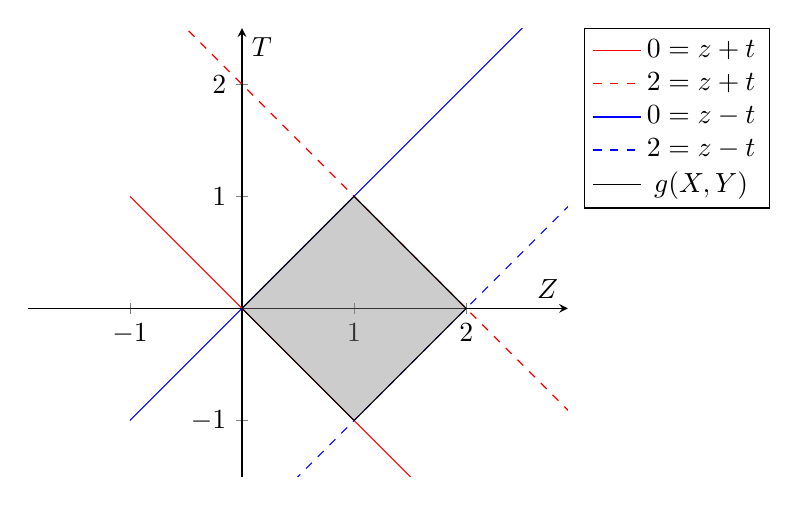
\begin{tikzpicture}
                \begin{axis}[
                    axis lines=middle,
                    xmin=-1.5, xmax=2.5,
                    ymin=-1.5, ymax=2.5,
                    xlabel={$Z$},
                    ylabel={$T$},
                    legend pos=outer north east, % Cambia la posición de la leyenda
                    axis equal,
                ]
                    % Recta 0=z+t
                    \addplot[domain=-1:3, samples=2, color=red]{-x};
                    \addlegendentry{$0=z+t$}
                    % Recta 2=z+t
                    \addplot[domain=-1:3, samples=2, color=red, dashed]{2-x};
                    \addlegendentry{$2=z+t$}
                    % Recta 0=z-t
                    \addplot[domain=-1:3, samples=2, color=blue]{x};
                    \addlegendentry{$0=z-t$}
                    % Recta 2=z-t
                    \addplot[domain=-1:3, samples=2, color=blue, dashed]{x-2};
                    \addlegendentry{$2=z-t$}

                    % Relleno
                    \addplot[fill=gray, fill opacity=0.4] coordinates {(0,0) (1,1) (2,0) (1,-1) (0,0)};
                    \addlegendentry{$g(X,Y)$}

                \end{axis}
            \end{tikzpicture}
        \end{figure}
        
        Buscamos ahora la función de densidad de probabilidad de $(Z,T)$:
        \begin{align*}
            f_{(Z,T)}(z, t)&=f_{(X,Y)}\left(\dfrac{z+t}{2},\dfrac{z-t}{2}\right)\cdot \left|\det Jg^{-1}(z,t)\right|
            =\\&= \begin{cases}
                k\cdot \dfrac{1}{2} & (z,t)\in g(X,Y), \\
                0 & \text{en otro caso}.
            \end{cases}
        \end{align*}

        Por tanto, la función de densidad de probabilidad de $(Z,T)$ es:
        \begin{equation*}
            f_{(Z,T)}(z, t) = \begin{cases}
                \dfrac{1}{2} & 0<z+t<2,~0<z-t<2, \\
                0 & \text{en otro caso}.
            \end{cases}
        \end{equation*}

        \item Determinar las funciones de densidad de probabilidad marginales del vector transformado $(Z,T)$.
        
        Para $z\in [0,2]$, tenemos que:
        \begin{align*}
            f_Z(z)&=\int_{-\infty}^{+\infty} f_{(Z,T)}(z, t) \, dt
        \end{align*}

        Los límites de integración los vemos claros en la gráfica anterior. Distinguimos en función del valor de $z$:
        \begin{itemize}
            \item Si $z\in [0,1]$, entonces:
            \begin{align*}
                f_Z(z)&=\int_{-z}^{z} \dfrac{1}{2} \, dt = \dfrac{1}{2}\left[t\right]_{-z}^z = \dfrac{1}{2}(z-(-z)) = z.
            \end{align*}

            \item Si $z\in [1,2]$, entonces:
            \begin{align*}
                f_Z(z)&=\int_{z-2}^{2-z} \dfrac{1}{2} \, dt = \dfrac{1}{2}\left[t\right]_{z-2}^{2-z} = \dfrac{1}{2}(2-z-(z-2)) = \dfrac{1}{2}(4-2z) = 2-z.
            \end{align*}
        \end{itemize}

        Por tanto, la función de densidad de probabilidad de $Z$ es:
        \begin{equation*}
            f_Z(z) = \begin{cases}
                z & 0<z<1, \\
                2-z & 1<z<2, \\
                0 & \text{en otro caso}.
            \end{cases}
        \end{equation*}

        Para $t\in [-1,1]$, tenemos que:
        \begin{align*}
            f_T(t)&=\int_{-\infty}^{+\infty} f_{(Z,T)}(z, t) \, dz
        \end{align*}

        Los límites de integración los vemos claros en la gráfica anterior. Distinguimos en función del valor de $t$:
        \begin{itemize}
            \item Si $t\in [-1,0]$, entonces:
            \begin{align*}
                f_T(t)&=\int_{-t}^{2+t} \dfrac{1}{2} \, dz = \dfrac{1}{2}\left[z\right]_{-t}^{2+t} = \dfrac{1}{2}(2+t-(-t)) = 1+t.
            \end{align*}

            \item Si $t\in [0,1]$, entonces:
            \begin{align*}
                f_T(t)&=\int_{t}^{2-t} \dfrac{1}{2} \, dz = \dfrac{1}{2}\left[z\right]_{t}^{2-t} = \dfrac{1}{2}(2-t-t) = 1-t.
            \end{align*}
        \end{itemize}

        Por tanto, la función de densidad de probabilidad de $T$ es:
        \begin{equation*}
            f_T(t) = \begin{cases}
                1+t & -1<t<0, \\
                1-t & 0<t<1, \\
                0 & \text{en otro caso}.
            \end{cases}
        \end{equation*}
        

        \item Determinar la función de distribución de probabilidad de $\nicefrac{X}{Y}$ y $XY$.
        % Hasta aquí hecho en clase. Preguntar a Joaquín

        Definimos la transformación:
        \Func{g}{\bb{R}^2}{\bb{R}^2}{(X,Y)}{(Z,T)=(\nicefrac{X}{Y},XY)}

        Para obtener $g^{-1}$, buscamos obtener $X,Y$ en función de $Z,T$:
        \begin{equation*}
            \left\{\begin{aligned}
                Z&=\nicefrac{X}{Y}, \\
                T&=XY.
            \end{aligned}\right\}\Longrightarrow
            \left\{\begin{aligned}
                X&=ZY=\sqrt{ZT}, \\
                Y&=\sqrt{\nicefrac{T}{Z}}.
            \end{aligned}\right.
        \end{equation*}
        Como $X,Y>0$, entonces $Z,T>0$, por lo que la inversa está bien definida.
        \Func{g^{-1}}{\bb{R}^+\times \bb{R}^+}{\bb{R}^2}{(Z,T)}{(X,Y)=(\sqrt{ZT},\sqrt{\nicefrac{T}{Z}})}

        Tenemos que todas las componentes de $g^{-1}$ son derivables:
        \begin{align*}
            \dfrac{\partial X}{\partial Z}(Z,T)&=\dfrac{T}{2\sqrt{ZT}}=\dfrac{\sqrt{T}}{2\sqrt{Z}}, & \dfrac{\partial X}{\partial T}(Z,T)&=\dfrac{\sqrt{Z}}{2\sqrt{T}},\\
            \dfrac{\partial Y}{\partial Z}(Z,T)&=\dfrac{-\frac{T}{Z^2}}{2\sqrt{\nicefrac{T}{Z}}}=-\dfrac{\sqrt{T}}{2Z\sqrt{Z}}, & \dfrac{\partial Y}{\partial T}(Z,T)&=\dfrac{1}{2Z\sqrt{\nicefrac{T}{Z}}}=\dfrac{1}{2\sqrt{TZ}}.
        \end{align*}

        Además, tenemos que:
        \begin{equation*}
            \det Jg^{-1}(z,t)=\begin{vmatrix}
                \dfrac{\sqrt{T}}{2\sqrt{Z}} & \dfrac{\sqrt{Z}}{2\sqrt{T}} \\
                -\dfrac{\sqrt{T}}{2Z\sqrt{Z}} & \dfrac{1}{2\sqrt{TZ}}
            \end{vmatrix}=\dfrac{1}{4Z}+\dfrac{1}{4Z}=\frac{1}{2Z}>0 \qquad \forall (z,t)\in\bb{R}^+\times \bb{R}^+.
        \end{equation*}

        Por tanto, $(Z,T)=g(X,Y)$ es un vector aleatorio continuo. Estudiamos ahora el conjunto $g(X,Y)$:
        \begin{align*}
            g(X,Y)&=\left\{(z,t)\in \bb{R}^+\times \bb{R}^+\mid 0<\sqrt{ZT}<1,~0<\sqrt{\nicefrac{T}{Z}}<1\right\}
            =\\&= \left\{(z,t)\in \bb{R}^+\times \bb{R}^+\mid 0<ZT<1,~0<T<Z\right\}
        \end{align*}

        Veamos el conjunto $g(X,Y)$ gráficamente:
        \begin{figure}[H]
            \centering
            \begin{tikzpicture}
                \begin{axis}[
                    axis lines=middle,
                    xmin=-1.5, xmax=2.5,
                    ymin=-1.5, ymax=2.5,
                    xlabel={$Z$},
                    ylabel={$T$},
                    legend pos=outer north east, % Cambia la posición de la leyenda
                    axis equal,
                ]
                    % Recta 0=z*t
                    \addplot[domain=-2:3, samples=2, color=red, dashed]{0};
                    \draw[red, dashed] (axis cs:0,-3) -- (axis cs:0,3);
                    \addlegendentry{$0=ZT$}
                    % Recta 1=z*t
                    \addplot[domain=-2:3, samples=100, color=red, name path=B]{1/x};
                    \addlegendentry{$1=ZT$}
                    % Recta 0=t
                    \addplot[name path=A, domain=-2:3, samples=2, color=blue, dashed]{0};
                    \addlegendentry{$0=T$}
                    % Recta z=t
                    \addplot[domain=-2:3, samples=2, color=blue, name path=C]{x};
                    \addlegendentry{$T=Z$}

                    % Marca del punto (1,1)
                    \addplot[color=black, mark=*, only marks, forget plot] coordinates {(1,1)};
                    \node[anchor=west] at (axis cs:1,1) {$(1,1)$};

                    % Relleno
                    \addplot [
                        thick,
                        color=orange,
                        fill=orange,
                        fill opacity=0.4
                    ]
                    fill between [
                        of=C and A,
                        soft clip={domain=0:1},
                    ];
                    \addplot [
                        thick,
                        color=orange,
                        fill=orange,
                        fill opacity=0.4
                    ]
                    fill between [
                        of=B and A,
                        soft clip={domain=1:4},
                    ];
                \addlegendentry{$g(X,Y)$}

                \end{axis}
            \end{tikzpicture}
        \end{figure}

        Buscamos ahora la función de densidad de probabilidad de $(Z,T)$:
        \begin{align*}
            f_{(Z,T)}(z, t)&=f_{(X,Y)}\left(\sqrt{ZT},\sqrt{\nicefrac{T}{Z}}\right)\cdot \left|\det Jg^{-1}(z,t)\right|
            =\\&= \begin{cases}
                \dfrac{1}{2z} & (z,t)\in g(X,Y), \\
                0 & \text{en otro caso}.
            \end{cases}
        \end{align*}

        Por tanto, la función de densidad de probabilidad de $(Z,T)$ es:
        \begin{equation*}
            f_{(Z,T)}(z, t) = \begin{cases}
                \dfrac{1}{2z} & 0<ZT<1,~0<T<Z, \\
                0 & \text{en otro caso}.
            \end{cases}
        \end{equation*}

        Para obtener la función de densidad de probabilidad de $Z=\nicefrac{X}{Y}$, tenemos que:
        \begin{align*}
            f_{Z}(z)&=\int_{-\infty}^{+\infty} f_{(Z,T)}(z, t) \, dt
        \end{align*}

        Los límites de integración los vemos claros en la gráfica anterior. Distinguimos en función del valor de $z$:
        \begin{itemize}
            \item Si $z\in [0,1]$, entonces:
            \begin{align*}
                f_Z(z)&=\int_{0}^{z} \dfrac{1}{2z} \, dt = \dfrac{1}{2z}\left[t\right]_{0}^{z} = \dfrac{1}{2z}z = \dfrac{1}{2}.
            \end{align*}

            \item Si $z\in \left[1,+\infty\right[$, entonces:
            \begin{align*}
                f_Z(z)&=\int_{0}^{\nicefrac{1}{z}} \dfrac{1}{2z} \, dt = \dfrac{1}{2z}\left[t\right]_{0}^{\nicefrac{1}{z}} = \dfrac{1}{2z^2}.
            \end{align*}
        \end{itemize}

        Por tanto, la función de densidad de probabilidad de $Z$ es:
        \begin{equation*}
            f_Z(z) = \begin{cases}
                \dfrac{1}{2} & 0<z<1, \\ \\
                \dfrac{1}{2z^2} & 1<z, \\
                0 & \text{en otro caso}.
            \end{cases}
        \end{equation*}

        Para obtener la función de densidad de probabilidad de $T=XY$, tenemos que:
        \begin{align*}
            f_{T}(t)&=\int_{-\infty}^{+\infty} f_{(Z,T)}(z, w) \, dz
        \end{align*}

        Los límites de integración los vemos claros en la gráfica anterior. Para $t\in \left]0,1\right]$, tenemos que:
        \begin{align*}
            f_T(t)&=\int_{t}^{\nicefrac{1}{t}} \dfrac{1}{2z} \, dz = \dfrac{1}{2}\left[\ln(z)\right]_{t}^{\nicefrac{1}{t}} = \dfrac{1}{2}\left[\ln\left(\nicefrac{1}{t}\right)-\ln(t)\right]
            = \dfrac{1}{2}\left[\ln(1)-2\ln(t)\right] = -\ln(t)
        \end{align*}

        Por tanto, la función de densidad de probabilidad de $T$ es:
        \begin{equation*}
            f_T(t) = \begin{cases}
                -\ln(t) & 0<t<1, \\
                0 & \text{en otro caso}.
            \end{cases}
        \end{equation*}

        Una vez tenemos ambas marginales, es fácil obtener la función de distribución de cada una.
        Respecto de $Z$, distinguimos en función del valor de $z$:
        \begin{itemize}
            \item Si $z\in [0,1]$, entonces:
            \begin{align*}
                F_Z(z)&=\int_{-\infty}^{z} f_Z(z) \, dz = \int_{0}^{z} \dfrac{1}{2} \, dz = \dfrac{1}{2}\left[z\right]_{0}^{z} = \dfrac{z}{2}
            \end{align*}

            \item Si $z\in \left[1,+\infty\right[$, entonces:
            \begin{align*}
                F_Z(z)&=\int_{-\infty}^{z} f_Z(z) \, dz = \int_{0}^{1} \dfrac{1}{2} \, dz + \int_{1}^{z} \dfrac{1}{2z^2} \, dz
                = \dfrac{1}{2} - \dfrac{1}{2}\left[\frac{1}{z}\right]_{1}^{z}
                =\\&= \dfrac{1}{2} - \dfrac{1}{2}\left(\frac{1}{z}-1\right)
                = 1-\dfrac{1}{2z}
            \end{align*}        
        \end{itemize}

        Por tanto, la función de distribución de probabilidad de $Z=\nicefrac{X}{Y}$ es:
        \begin{equation*}
            F_Z(z) = \begin{cases}
                \dfrac{z}{2} & 0<z<1, \\ \\
                1-\dfrac{1}{2z} & 1<z, \\
                0 & \text{en otro caso}.
            \end{cases}
        \end{equation*}

        Respecto de $T$, para $t\in \left]0,1\right]$, tenemos que:
        \begin{align*}
            F_T(t)&=\int_{-\infty}^{t} f_T(t) \, dt = \int_{0}^{t} -\ln(t) \, dt = -\left[t\ln(t)-t\right]_{0}^{t} =\\&=
            -t\ln(t)+t +\lim_{t\to 0}t\ln(t) = -t\ln(t)+t
        \end{align*}

        Por tanto, la función de distribución de probabilidad de $T=XY$ es:
        \begin{equation*}
            F_T(t) = \begin{cases}
                0 & t\leq 0, \\
                -t\ln(t)+t & 0<t<1, \\
                1 & 1\leq t, \\
            \end{cases}
        \end{equation*}


        \item Determinar la función de distribución de probabilidad de $\max(X,Y)$, y del $\min(X,Y)$.
        
        Dado $x\in \bb{R}$, tenemos que:
        \begin{equation*}
            P[\max(X,Y)\leq x]=P[X\leq x,Y\leq x] = P[(X,Y)\leq (x,x)]
        \end{equation*}

        Calculamos por tanto dicho valor sabiendo $f_{(X,Y)}$. Para $z\in [0,1]$, tenemos que:
        \begin{align*}
            P[(X,Y)\leq (z,z)]&=\int_{0}^{z}\int_{0}^{z} k \, dy \, dx = k\int_{0}^{z} z \, dx
            = kz\left[x\right]_{0}^{z} = kz^2 = z^2
        \end{align*}

        Por tanto, la función de distribución de probabilidad de $\max(X,Y)$ es:
        \begin{equation*}
            F_{\max(X,Y)}(z) = \begin{cases}
                0 & z\leq 0, \\
                z^2 & 0<z<1, \\
                1 & 1\leq z.
            \end{cases}
        \end{equation*}

        Respecto del $\min(X,Y)$, dado $z\in \bb{R}$, tenemos que:
        \begin{equation*}
            P[\min(X,Y)\leq z]=1-P[\min(X,Y)>z]=1-P[(X,Y)>z]
        \end{equation*}

        Calculamos dicho valor sabiendo $f_{(X,Y)}$. Distinguimos en función de $z$:
        \begin{itemize}
            \item Si $z\leq 0$, entonces $P[(X,Y)>z]=1$.

            \item Si $0<z<1$, entonces:
            \begin{align*}
                P[(X,Y)>z]&=\int_{z}^{1}\int_{z}^{1} k \, dy \, dz = k\int_{z}^{1} (1-z) \, dz
                = k(1-z)\left[x\right]_{z}^{1} = (1-z)^2
            \end{align*}

            \item Si $z\geq 1$, entonces $P[(X,Y)>z]=0$.
        \end{itemize}

        Por tanto, la función de distribución de probabilidad de $\min(X,Y)$ es:
        \begin{equation*}
            F_{\min(X,Y)}(z) = 1-P[(X,Y)>z]=\begin{cases}
                0 & z\leq 0, \\
                1-(1-z)^2 & 0<z<1, \\
                1 & 1\leq z.
            \end{cases}
        \end{equation*}

        \item Determinar la función de distribución de probabilidad conjunta del $\max(X,Y)$, y del $\min(X,Y)$.
        
        Dado $z,t\in \bb{R}$, distinguimos casos:
        \begin{itemize}
            \item Si $z\leq t$, como $\min (X,Y)\leq \max(X,Y)$, entonces:
            \begin{align*}
                P[\max(X,Y)\leq z,\min(X,Y)\leq t]&=P[\max(X,Y)\leq z] = F_{\max(X,Y)}(z)
            \end{align*}

            Distinguimos en función de $z$:
            \begin{itemize}
                \item Si $z\leq 0$, entonces $F_{\max(X,Y)}(z)=0$.
                \item Si $0<z<1$, entonces $F_{\max(X,Y)}(z)=z^2$.
                \item Si $z\geq 1$, entonces $F_{\max(X,Y)}(z)=1$.
            \end{itemize}

            \item Si $z>t$, entonces:
            \begin{align*}
                P[\max(X,Y)\leq z,&\min(X,Y)\leq t]
                \\&=P[\max(X,Y)\leq z]-P[\max(X,Y)\leq z,\min(X,Y)> t]
                =\\&= P[\max(X,Y)\leq z]-P[t<X\leq z,t<Y\leq z]
            \end{align*}

            Distinguimos en función de $z$:
            \begin{itemize}
                \item Si $z\leq 0$, entonces $P[\max(X,Y)\leq z]=0$. Además, $t<z\leq 0$. Por tanto:
                \begin{equation*}
                    P[t<X\leq z,t<Y\leq z]=0
                \end{equation*}
                Por tanto, $P[\max(X,Y)\leq z,\min(X,Y)\leq t]=0$.

                \item Si $0<z<1$, entonces $P[\max(X,Y)\leq z]=z^2$. Además, sabemos que $t<z<1$. Distinguimos en función de $t$:
                \begin{itemize}
                    \item Si $t\leq 0$, entonces:
                    \begin{align*}
                        P[t<X\leq z,t<Y\leq z]&=\int_{0}^{z}\int_{0}^{z} k \, dy \, dx = kz^2 = z^2
                    \end{align*}
                    Por tanto, $P[\max(X,Y)\leq z,\min(X,Y)\leq t]=z^2-z^2=0$.
                    \item Si $0<t<z$, entonces:
                    \begin{align*}
                        P[t<X\leq z,t<Y\leq z]&=\int_{t}^{z}\int_{t}^{z} k \, dy \, dx = k(z-t)^2 = (z-t)^2
                    \end{align*}
                    Por tanto, tenemos que:
                    $$P[\max(X,Y)\leq z,\min(X,Y)\leq t]=z^2-(z-t)^2=z^2-z^2+2zt-t^2=2zt-t^2$$
                \end{itemize}
                \item Si $z\geq 1$, entonces $P[\max(X,Y)\leq z]=1$. Distinguimos en función de $t$:
                \begin{itemize}
                    \item Si $t\leq 0$, entonces:
                    \begin{align*}
                        P[t<X\leq z,t<Y\leq z]&=\int_{0}^{1}\int_{0}^{1} k \, dy \, dx = k = 1
                    \end{align*}
                    Por tanto, $P[\max(X,Y)\leq z,\min(X,Y)\leq t]=1-1=0$.
                    \item Si $0<t<1$, entonces:
                    \begin{align*}
                        P[t<X\leq z,t<Y\leq z]&=\int_{t}^{1}\int_{t}^{1} k \, dy \, dx = k(1-t)^2 = (1-t)^2
                    \end{align*}
                    Por tanto, $$P[\max(X,Y)\leq z,\min(X,Y)\leq t]=1-(1-t)^2=1-1+2t-t^2=2t-t^2$$
                    \item Si $t\geq 1$, $t<z$, entonces:
                    \begin{align*}
                        P[t<X\leq z,t<Y\leq z]&=0
                    \end{align*}
                    Por tanto, $P[\max(X,Y)\leq z,\min(X,Y)\leq t]=1-0=1$.
                \end{itemize}
            \end{itemize}
        \end{itemize}
        
            
        Por tanto, la función de distribución de probabilidad conjunta de $\max(X,Y)$ y $\min(X,Y)$ es:
        \begin{equation*}
            F_{\max(X,Y),\min(X,Y)}(z,t) = \begin{cases}
                0 & z\leq 0 \lor t\leq 0\qquad (R_0), \\
                z^2 & z\leq t \land 0<z<1 \qquad (R_1), \\
                2zt-t^2 & 0<t<z<1 \qquad (R_2), \\
                2t-t^2 & 0<t<1\leq z \qquad (R_3), \\
                1 & 1\leq t\land 1\leq z \qquad (R_4).
            \end{cases}
        \end{equation*}

        Veamos gráficamente cada una de las regiones:
        \begin{figure}[H]
            \centering
            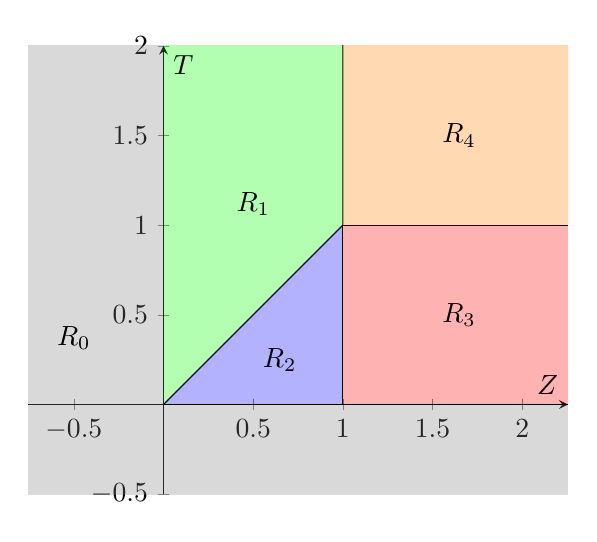
\begin{tikzpicture}
                \begin{axis}[
                    axis lines=middle,
                    xmin=-0.5, xmax=2,
                    ymin=-0.5, ymax=2,
                    xlabel={$Z$},
                    ylabel={$T$},
                    legend pos=outer north east, % Cambia la posición de la leyenda
                    axis equal,
                ]
                    % R0: (0,5) (-5,5) (-5,-5) (5,-5) (5,0) (0,0)
                    \addplot[fill=gray, fill opacity=0.3] coordinates {(0,5) (-5,5) (-5,-5) (5,-5) (5,0) (0,0)};
                    \node[anchor=south] at (-0.5,0.25) {$R_0$};

                    % R1: (0,0) (1,1) (1,5) (0,5)
                    \addplot[fill=green, fill opacity=0.3] coordinates {(0,0) (1,1) (1,5) (0,5)};
                    \node[anchor=south] at (0.5,1) {$R_1$};

                    % R2: (0,0) (1,0) (1,1)
                    \addplot[fill=blue, fill opacity=0.3] coordinates {(0,0) (1,0) (1,1)};
                    \node[anchor=west] at (axis cs:0.5,0.25) {$R_2$};

                    % R3: (1,0) (1,1) (5,1) (5,0)
                    \addplot[fill=red, fill opacity=0.3] coordinates {(1,0) (1,1) (5,1) (5,0)};
                    \node[anchor=west] at (axis cs:1.5,0.5) {$R_3$};

                    % R4: (1,1) (5,1) (5,5) (1,5)
                    \addplot[fill=orange, fill opacity=0.3] coordinates {(1,1) (5,1) (5,5) (1,5)};
                    \node[anchor=west] at (axis cs:1.5,1.5) {$R_4$};
                    
                \end{axis}
            \end{tikzpicture}
        \end{figure}
    \end{enumerate}
\end{ejercicio}

\begin{ejercicio}
    Sea $(X,Y)$ un vector aleatorio bidimensional discreto, cuya función masa de probabilidad conjunta se calcula como el producto de las funciones masa de probabilidad marginales de $X$ e $Y$. Las variables aleatorias $X$ e $Y$ se distribuyen según una Poisson con parámetro $\lambda>0$. Calcular la función de distribución de probabilidad marginal del máximo y del mínimo, así como la distribución conjunta del máximo y del mínimo.\\

    Tenemos que:
    \begin{equation*}
        P[X=x,Y=y] = P[X=x]\cdot P[Y=y]
    \end{equation*}

    Como $X,Y\sim \cc{P}(\lm)$, tenemos que:
    \begin{align*}
        P[X=x,Y=y]&=P[X=x]\cdot P[Y=y]
        =\\&= \dfrac{e^{-\lm}\lm^x}{x!}\cdot \dfrac{e^{-\lm}\lm^y}{y!}
        =\\&= \dfrac{e^{-2\lm}\lm^{x+y}}{x!y!}
    \end{align*}

    Calculemos la marginal del máximo. Para $n\in \bb{N}$, tenemos que:
    \begin{align*}
        P[\max(X,Y)\leq n]&=P[X\leq n,Y\leq n]
        = P[(X,Y)\leq (n,n)]
        =\\&= \sum_{i=0}^{n}\sum_{j=0}^{n}P[X=i,Y=j]
        =\\&= \sum_{i=0}^{n}\sum_{j=0}^{n}\dfrac{e^{-2\lm}\lm^{i+j}}{i!j!}
        =\\&= e^{-2\lm}\sum_{i=0}^{n}\sum_{j=0}^{n}\dfrac{\lm^{i+j}}{i!j!}
        = e^{-2\lm}\sum_{i=0}^{n}\dfrac{\lm^i}{i!}\sum_{j=0}^{n}\dfrac{\lm^j}{j!}
        =\\&= P[X\leq n]\cdot P[Y\leq n]
    \end{align*}

    Calculamos la marginal del mínimo. Para $n\in \bb{N}$, tenemos que:
    \begin{align*}
        P[\min(X,Y)\leq n]&=1-P[\min(X,Y)>n]
        =\\&= 1-P[X>n,Y>n]
        =\\&= 1-P[(X,Y)>(n,n)]
        =\\&= 1-\sum_{i=n+1}^{+\infty}\sum_{j=n+1}^{+\infty}P[X=i,Y=j]
        =\\&= 1-\sum_{i=n+1}^{+\infty}\sum_{j=n+1}^{+\infty}\dfrac{e^{-2\lm}\lm^{i+j}}{i!j!}
        =\\&= 1-e^{-2\lm}\sum_{i=n+1}^{+\infty}\sum_{j=n+1}^{+\infty}\dfrac{\lm^{i+j}}{i!j!}
        =\\&= 1-e^{-2\lm}\sum_{i=n+1}^{+\infty}\dfrac{\lm^i}{i!}\sum_{j=n+1}^{+\infty}\dfrac{\lm^j}{j!}
        =\\&= 1-P[X>n]\cdot P[Y>n]
    \end{align*}

    Calculamos ahora la distribución conjunta del máximo y del mínimo. Para los valores $n,m\in\bb{N}$, tenemos que:
    \begin{itemize}
        \item Si $n\leq m$, entonces:
        \begin{align*}
            P[\max(X,Y)\leq n,\min(X,Y)\leq m]&=P[\max(X,Y)\leq n]
        \end{align*}

        \item Si $m<n$, entonces:
        \begin{align*}
            P[\max(X,Y)&\leq n,\min(X,Y)\leq m]
            =\\&= P[\max(X,Y)\leq n]-P[\max(X,Y)\leq n,\min(X,Y)> m]
            =\\&= P[\max(X,Y)\leq n]-P[m<X\leq n,m<Y\leq n]
            =\\&= P[X\leq n]\cdot P[Y\leq n]-P[m+1\leq X\leq n,m+1<Y\leq n]
        \end{align*}

        Calculamos la probabilidad $P[m+1\leq X\leq n,m+1<Y\leq n]$:
        \begin{align*}
            P[m+1&\leq X\leq n,m+1<Y\leq n]=\sum_{i=m+1}^{n}\sum_{j=m+1}^{n}P[X=i,Y=j]
            =\\&= \sum_{i=m+1}^{n}\sum_{j=m+1}^{n}\dfrac{e^{-2\lm}\lm^{i+j}}{i!j!}
            =\\&= e^{-2\lm}\sum_{i=m+1}^{n}\sum_{j=m+1}^{n}\dfrac{\lm^{i+j}}{i!j!}
            =\\&= \sum_{i=m+1}^{n}e^{-\lm}\dfrac{\lm^i}{i!}\sum_{j=m+1}^{n}e^{-\lm}\dfrac{\lm^j}{j!}
            =\\&= \left(P[X\leq n]-P[X\leq m]\right)\left(P[Y\leq n]-P[Y\leq m]\right)
        \end{align*}

        Por tanto, la distribución conjunta del máximo y del mínimo es:
        \begin{multline*}
            P[\max(X,Y)\leq n,\min(X,Y)\leq m] =\\= \begin{cases}
                P[X\leq n]\cdot P[Y\leq n] & n\leq m, \\
                P[X\leq n]\cdot P[Y\leq n]-\left(P[X\leq n]-P[X\leq m]\right)\left(P[Y\leq n]-P[Y\leq m]\right) & m<n.
            \end{cases}
        \end{multline*}
    \end{itemize}
\end{ejercicio}

\begin{ejercicio}
    Sea $(X,Y)$ un vector aleatorio con función de densidad de probabilidad
    \begin{equation*}
        f(x, y) = \begin{cases}
            2 & 0<x<1,~0<y<x, \\
            0 & \text{en otro caso}.
        \end{cases}
    \end{equation*}
    Calcular la densidad de probabilidad de las variables $Z=aX+bY$, $T=\nicefrac{X}{Y}$, a partir de la densidad de probabilidad conjunta de $(Z,T)=(aX+bY,\nicefrac{X}{Y})$, $a,b>0$.\\

    Definimos la transformación:
    \Func{g}{E_{(X,Y)}}{\bb{R}^2}{(X,Y)}{(Z,T)=(aX+bY,\nicefrac{X}{Y})}

    Para obtener $g^{-1}$, buscamos obtener $X,Y$ en función de $Z,T$:
    \begin{equation*}
        \left\{\begin{aligned}
            Z&=aX+bY, \\
            T&=\nicefrac{X}{Y}.
        \end{aligned}\right\}\Longrightarrow
        \left\{\begin{aligned}
            X&=\dfrac{TZ}{aT+b}, \\
            Y&=\dfrac{Z}{aT+b}.
        \end{aligned}\right.
    \end{equation*}
    Notemos que $a,b>0$, y como $X,Y>0$, entonces $T>0$. Por tanto, $aT+b>0$, por lo que está bien definida la transformación.

    Por tanto, tenemos que:
    \Func{g^{-1}}{g(E_{(X,Y)})}{E_{(X,Y)}}{(Z,T)}{(X,Y)=\left(\dfrac{TZ}{aT+b},\dfrac{Z}{aT+b}\right)}

    Tenemos que todas las componentes de $g^{-1}$ son derivables:
    \begin{align*}
        \dfrac{\partial X}{\partial Z}(Z,T)&=\dfrac{T}{aT+b}, & \dfrac{\partial X}{\partial T}(Z,T)&=\dfrac{bZ}{(aT+b)^2},\\
        \dfrac{\partial Y}{\partial Z}(Z,T)&=\dfrac{1}{aT+b}, & \dfrac{\partial Y}{\partial T}(Z,T)&=\dfrac{-aZ}{(aT+b)^2}.
    \end{align*}

    Además, tenemos que:
    \begin{align*}
        \det Jg^{-1}(z,t)&=\begin{vmatrix}
            \dfrac{T}{aT+b} & \dfrac{bZ}{(aT+b)^2} \\
            \dfrac{1}{aT+b} & \dfrac{-aZ}{(aT+b)^2}
        \end{vmatrix}=\dfrac{1}{(aT+b)^4}\begin{vmatrix}
            T(aT+b) & bZ \\
            aT+b & -aZ
        \end{vmatrix}
        =\\&=\dfrac{1}{(aT+b)^4}(aT+b)(-TaZ -bZ)
        = -\dfrac{Z}{(aT+b)^2}\neq 0 \qquad \forall (z,t)\in g(E_{(X,Y)}).
    \end{align*}

    Por tanto, $(Z,T)=g(X,Y)$ es un vector aleatorio continuo. Veamos ahora el valor de $g(X,Y)$ para $X\in [0,1]$, $Y\in [0,X]$:
    \begin{align*}
        g(X,Y)&=\left\{(z,t)\in \bb{R}^2\mid 0<\dfrac{tz}{at+b}<1,~0<\dfrac{z}{at+b}<\dfrac{tz}{at+b}\right\}
        =\\&= \left\{(z,t)\in \bb{R}^2\mid 0<tz<at+b,~0<1<t\right\}
        =\\&= \left\{(z,t)\in \bb{R}^2\mid 0<z<a+\dfrac{b}{t},~1<t\right\}
    \end{align*}

    Veamos este conjunto gráficamente:
    \begin{figure}[H]
        \centering
        \begin{tikzpicture}
            \begin{axis}[
                axis lines=middle,
                xmin=-1, xmax=4,
                ymin=-1, ymax=4,
                xlabel={$Z$},
                ylabel={$T$},
                xtick=\empty,
                ytick=\empty,
                legend pos=outer north east, % Cambia la posición de la leyenda
                axis equal,
            ]   
                
                % Recta 1=t
                \addplot[name path=A, domain=-3:4, samples=2, color=blue]{1};
                \addlegendentry{$1=t$}
                % Hipérbola y=B/(x-A)
                \addplot[name path=B, domain=1:4, samples=100, color=red]{1/(x-1)};
                \addplot[domain=-3:0.9, samples=100, color=red, forget plot]{1/(x-1)};
                \addlegendentry{$z=a+\nicefrac{b}{t}$}

                % Asíntotas de la hipérbola
                \addplot[domain=-3:4, samples=2, color=red, dashed]{0};
                \draw[dashed, red] (axis cs:1,-2) -- (axis cs:1,4);

                % Indicamos que la asíntota es en z=a y en t=0
                \node[red, right] at (axis cs:1,-0.5) {$z=a$};
                \node[red, above left] at (axis cs:-0.5,0) {$t=0$};

                % Relleno entre la hipérbola y la recta
                \addplot [
                        thick,
                        color=orange,
                        fill=orange,
                        fill opacity=0.4
                    ]
                    fill between [
                        of=B and A,
                        soft clip={domain=1:2},
                    ];
                \addlegendentry{$g(X,Y)$}

                % Señalizamos el punto (a,1) y el punto (a+b,1)
                \node[circle,fill,inner sep=1pt, label=above left:{$(a,1)$}] at (axis cs:1,1) {};
                \node[circle,fill,inner sep=1pt, label=above right:{$(a+b,1)$}] at (axis cs:2,1) {};
            \end{axis}
        \end{tikzpicture}
    \end{figure}    

    La densidad de probabilidad de $(Z,T)$ es:
    \begin{align*}
        &f_{(Z,T)}(z, t) = f_{(X,Y)}\left(\dfrac{tz}{at+b},\dfrac{z}{at+b}\right)\cdot \left|- \dfrac{Z}{(aT+b)^2}\right|
        =\\&= \begin{cases}
            \dfrac{2z}{(at+b)^2} & (z,t)\in g(X,Y), \\
            0 & \text{en otro caso}.
        \end{cases}
    \end{align*}

    Por tanto, la densidad de probabilidad de $(Z,T)$ es:
    \begin{equation*}
        f_{(Z,T)}(z, t) = \begin{cases}
            \dfrac{2z}{(at+b)^2} & (z,t)\in g(X,Y), \\
            0 & \text{en otro caso}.
        \end{cases}
    \end{equation*}

    Calculemos ahora la densidad de probabilidad de $Z=aX+bY$. Para $z\in\left]a,a+b\right[$, tenemos que:
    \begin{align*}
        f_Z(z)&=\int_{-\infty}^{+\infty} f_{(Z,T)}(z, t) \, dt
        = \int_{1}^{\frac{b}{z-a}} \dfrac{2z}{(at+b)^2} \, dt
        =\\&= -\frac{2z}{a}\left[\dfrac{1}{at+b}\right]_{1}^{\frac{b}{z-a}}
        = -\frac{2z}{a}\left[\dfrac{1}{\frac{ba}{z-a}+b}-\dfrac{1}{a+b}\right]
        = -\frac{2z}{a}\left[\dfrac{z-a}{bz}-\dfrac{1}{a+b}\right]
        =\\&= -\frac{2\cancel{z}}{a}\left[\dfrac{(z-a)(a+b)-bz}{b\cancel{z}(a+b)}\right]
        = -\frac{2}{a}\left[\dfrac{az+\cancel{bz}-a^2-ab-\cancel{bz}}{b(a+b)}\right]
        =\\&= 2\cdot \left[\dfrac{a+b-z}{b(a+b)}\right]
    \end{align*}

    Por tanto, la densidad de probabilidad de $Z=aX+bY$ es:
    \begin{equation*}
        f_Z(z) = \begin{cases}
            2\cdot \left[\dfrac{a+b-z}{b(a+b)}\right] & z\in\left]a,a+b\right[, \\
            0 & \text{en otro caso}.
        \end{cases}
    \end{equation*}

    Calculemos ahora la densidad de probabilidad de $T=\nicefrac{X}{Y}$. Para $t>1$, tenemos que:
    \begin{align*}
        f_T(t)&=\int_{-\infty}^{+\infty} f_{(Z,T)}(z, t) \, dz
        = \int_{a}^{a+\frac{b}{t}} \dfrac{2z}{(at+b)^2} \, dz
        =\\&= \dfrac{1}{(at+b)^2}\left[z^2\right]_{a}^{a+\frac{b}{t}}
        = \dfrac{1}{(at+b)^2}\left[\left(a+\dfrac{b}{t}\right)^2-a^2\right]
        =\\&= \dfrac{1}{(at+b)^2}\left[\dfrac{2ab}{t}+\dfrac{b^2}{t^2}\right]
        = \dfrac{b}{(at+b)^2}\left[\dfrac{2at+b}{t^2}\right]
    \end{align*}

    Por tanto, la densidad de probabilidad de $T=\nicefrac{X}{Y}$ es:
    \begin{equation*}
        f_T(t) = \begin{cases}
            \dfrac{b}{(at+b)^2}\left[\dfrac{2at+b}{t^2}\right] & t>1, \\
            0 & \text{en otro caso}.
        \end{cases}
    \end{equation*}


\end{ejercicio}

\begin{ejercicio}
    Sea $(X,Y)$ un vector aleatorio, cuya función de densidad de probabilidad conjunta se calcula como producto de las funciones de densidad de probabilidad marginales de $X$ e $Y$, siendo $X\sim\exp(\lambda)$ e $Y\sim\exp(\mu)$. Calcular la función de distribución de probabilidad conjunta del vector aleatorio
    $$(Z,T)=(\min(X,Y),T),\qquad T=\begin{cases} 0 & Y<X \\ 1 & X<Y \end{cases}$$

    Como $X\sim \exp(\lm)$ e $Y\sim \exp(\mu)$, tenemos que:
    \begin{align*}
        f_X(x)&=\begin{cases}
            \lm e^{-\lm x} & x\geq 0, \\
            0 & x<0,
        \end{cases} & f_Y(y)&=\begin{cases}
            \mu e^{-\mu y} & y\geq 0, \\
            0 & y<0.
        \end{cases}
    \end{align*}

    Por tanto, la función de densidad de probabilidad conjunta de $(X,Y)$ es:
    \begin{align*}
        f_{(X,Y)}(x,y)&=f_X(x)\cdot f_Y(y)
        = \begin{cases}
            \lm\mu e^{-\lm x-\mu y} & x,y\geq 0, \\
            0 & \text{en otro caso}.
        \end{cases}
    \end{align*}

    Tenemos que $E_X=E_Y=\bb{R}^+$, por lo que $E_Z=\bb{R}^+$. Además, $E_T=\{0,1\}$.
    Tenemos por tanto la siguiente situación:
    \begin{figure}[H]
        \centering
        \begin{tikzpicture}
            \begin{axis}[
                axis lines=middle,
                xmin=-1, xmax=4,
                ymin=-1, ymax=2,
                xlabel={$Z$},
                ylabel={$T$},
                legend pos=outer north east, % Cambia la posición de la leyenda
                axis equal,
            ]   
                
                % Recta 1=t
                \addplot[name path=A, domain=-3:4, samples=2, color=blue, thick]{1};
                \addlegendentry{$T=1$}
                % Recta 0=t
                \addplot[name path=B, domain=-3:4, samples=2, color=blue, thick, dashed]{0};
                \addlegendentry{$T=0$}

                % Zona 0:Triángulo (0,0) (0,5) (-5,5) (-5,-5) (5,-5) (5,0)
                \fill[red, opacity=0.2] (0,0) -- (0,5) -- (-5,5) -- (-5,-5) -- (5,-5) -- (5,0) -- cycle;
                \node at (-0.5,-0.5) {$R_0$};

                % Zona 1:Triángulo (0,0) (5,0) (5,1) (0,1)
                \fill[green, opacity=0.2] (0,0) -- (5,0) -- (5,1) -- (0,1) -- cycle;
                \node at (1.5,0.5) {$R_1$};
                
                % Zona 2:Triángulo (0,1) (0,5) (5,5) (5,1)
                \fill[orange, opacity=0.2] (0,1) -- (0,5) -- (5,5) -- (5,1) -- cycle;
                \node at (1.5,1.5) {$R_2$};
            \end{axis}
        \end{tikzpicture}
    \end{figure}

    Calculamos la función de distribución de probabilidad conjunta de $(Z,T)$:
    \begin{align*}
        P[Z\leq z,T\leq t]&=P[\min(X,Y)\leq z,T\leq t]
    \end{align*}

    Dados $z,t\in \bb{R}$, distinguimos casos:
    \begin{itemize}
        \item Si $z\leq 0$ o $t<0$, (es decir, $(z,t)\in R_0$), entonces:
        \begin{equation*}
            P[\min(X,Y)\leq z,T\leq t]=0
        \end{equation*}

        \item Si $z>0$ y $t\in \left[0,1\right[$, (es decir, $(z,t)\in R_1$), entonces:
        \begin{align*}
            P[\min(X,Y)\leq z,T\leq t]&=P[\min(X,Y)\leq z,T=0]
            = P[\min(X,Y)\leq z,Y<X]
            =\\&= P[Y\leq z,Y<X]
            = \int_{0}^{z}\int_{y}^{+\infty} f_{(X,Y)}(x,y) \, dx \, dy
            =\\&= \int_{0}^{z}\int_{y}^{+\infty} \lm\mu e^{-\lm x-\mu y} \, dx \, dy
            = \int_{0}^{z}\mu e^{-\mu y}\int_{y}^{+\infty} \lm e^{-\lm x} \, dx \, dy
            =\\&= \int_{0}^{z}\mu e^{-\mu y}\left[-e^{-\lm x}\right]_{y}^{+\infty} \, dy
            = \int_{0}^{z}\mu e^{-\mu y}e^{-\lm y} \, dy
            =\\&= \mu\int_{0}^{z} e^{-(\lm+\mu)y} \, dy
            = \mu\left[\dfrac{e^{-(\lm+\mu)y}}{-(\lm+\mu)}\right]_{0}^{z}
            =\\&= -\dfrac{\mu}{\lm+\mu} \left[\exp(-(\lm+\mu)z)-1\right]
        \end{align*}

        \item Si $z>0$ y $t\geq 1$, (es decir, $(z,t)\in R_2$), entonces:
        
        Tenemos dos opciones para calcular $P[\min(X,Y)\leq z,T\leq t]$:
        \begin{description}
            \item[Opción 1)] Como $E_T=\{0,1\}$, sabemos que:
            \begin{align*}
                P[\min(X,Y)\leq z,T\leq t]&=P[\min(X,Y)\leq z]
            \end{align*}

            Por tanto, calculamos $P[\min(X,Y)\leq z]$:
            \begin{align*}
                P[\min(X,Y)\leq z] &= 1-P[\min(X,Y)>z] = 1-P[X>z,Y>z]
                =\\&= 1-\int_{z}^{+\infty}\int_{z}^{+\infty} f_{(X,Y)}(x,y) \, dy \, dx
                =\\&= 1-\int_{z}^{+\infty}\int_{z}^{+\infty} \lm\mu e^{-\lm x-\mu y} \, dy \, dx
                =\\&= 1-\int_{z}^{+\infty}\lm e^{-\lm x}\, dx \, \int_{z}^{+\infty} \mu e^{-\mu y} \, dy
                =\\&= 1-\left[-e^{-\lm x}\right]_{z}^{+\infty}\left[-e^{-\mu y}\right]_{z}^{+\infty}
                = 1-\left[e^{-\lm z}-0\right]\left[e^{-\mu z}-0\right]
                =\\&= 1-(e^{-\lm z})(e^{-\mu z})
                = 1-\exp(-(\lm+\mu)z)
            \end{align*}

            \item[Opción 2)] Como $E_T=\{0,1\}$, sabemos que:
            \begin{align*}
                P[\min(X,Y)\leq z,T\leq t]&=P[\min(X,Y)\leq z,T=0] + P[\min(X,Y)\leq z,T=1]
            \end{align*}

            La primera ya la hemos obtenido anteriormente. por tanto, calculamos la segunda probabilidad:
            \begin{align*}
                P[\min(X,Y)\leq z,T=1]&=P[\min(X,Y)\leq z,X<Y] = P[X\leq z,X<Y]
                =\\&= \int_{0}^{z}\int_{x}^{+\infty} f_{(X,Y)}(x,y) \, dy \, dx
                = \int_{0}^{z}\int_{x}^{+\infty} \lm\mu e^{-\lm x-\mu y} \, dy \, dx
                =\\&= \int_{0}^{z}\lm e^{-\lm x}\int_{x}^{+\infty} \mu e^{-\mu y} \, dy \, dx
                = \int_{0}^{z}\lm e^{-\lm x}\left[-e^{-\mu y}\right]_{x}^{+\infty} \, dx
                =\\&= \int_{0}^{z}\lm e^{-\lm x}e^{-\mu x} \, dx
                = \lm\int_{0}^{z} e^{-(\lm+\mu)x} \, dx
                = \lm\left[\dfrac{e^{-(\lm+\mu)x}}{-(\lm+\mu)}\right]_{0}^{z}
                =\\&= -\dfrac{\lm}{\lm+\mu} \left[\exp(-(\lm+\mu)z)-1\right]
            \end{align*}

            Sumando ambos resultados, tenemos que:
            \begin{align*}
                P[\min(X,Y)\leq z,T\leq t]&= [\exp(-(\lm+\mu)z)-1]\left(-\dfrac{\mu}{\lm+\mu} -\dfrac{\lm}{\lm+\mu}\right)
                =\\&= 1-\exp(-(\lm+\mu)z)
            \end{align*}
        \end{description}
    \end{itemize}

    En cualquier caso, la función de distribución de probabilidad conjunta $(Z,T)$ es:
    \begin{equation*}
        F_{(Z,T)}(z,t) = \begin{cases}
            0 & z\leq 0 \text{ o } t<0, \\
            -\dfrac{\mu}{\lm+\mu} \left[\exp(-(\lm+\mu)z)-1\right] & z>0 \text{ y } t\in \left[0,1\right[, \\
            1-\exp(-(\lm+\mu)z) & z>0 \text{ y } t\geq 1.
        \end{cases}
    \end{equation*}
\end{ejercicio}

\begin{ejercicio}
    Sea $(X,Y)$ un vector aleatorio, cuya función de densidad de probabilidad conjunta se calcula como en el problema anterior, considerando $\lambda=\mu$. Calcular la distribución de probabilidad de:
    \begin{enumerate}
        \item $|X-Y|$,

        Del apartado anterior, tenemos que:
        \begin{equation*}
            f_{(X,Y)}(x,y)=\begin{cases}
                \lm^2 e^{-\lm(x+y)} & x,y\geq 0, \\
                0 & \text{en otro caso}.
            \end{cases}
        \end{equation*}

        Buscamos calcular $P[|X-Y|\leq z]$ para todo $z\in\bb{R}$.
        Si $z\leq 0$, tenemos que $P[|X-Y|\leq z]=0$, por lo que sea $z\in \bb{R}^+$.
        Tenemos que:
        \begin{align*}
            P[|X-Y|\leq z]&=P[-z\leq X-Y\leq z]
        \end{align*}

        Sabiendo que $X,Y\geq 0$, tenemos que la situación es la descrita en la Figura~\ref{fig:|X-Y|_z}.
        \begin{figure}
            \centering
            \begin{tikzpicture}
                \begin{axis}[
                    axis lines=middle,
                    xmin=-1, xmax=4,
                    ymin=-1, ymax=4,
                    xlabel={$X$},
                    ylabel={$Y$},
                    legend pos=outer north east, % Cambia la posición de la leyenda
                    axis equal,
                ]
                    % Definimos la variable z>0
                    \def\z{1}
                    
                    % Recta X-Y=-z
                    \addplot[name path=A, domain=-3:4, samples=2, color=blue, thick]{x+\z};
                    \addlegendentry{$X-Y=-z$}
                    % Recta X-Y=z
                    \addplot[name path=B, domain=-3:4, samples=2, color=blue, thick, dashed]{x-\z};
                    \addlegendentry{$X-Y=z$}

                    % Relleno entre las rectas
                    \addplot [
                        thick,
                        color=orange,
                        fill=orange,
                        fill opacity=0.4
                    ]
                    fill between [
                        of=A and B,
                        soft clip={domain=1:4},
                    ];

                    % Relleno (0,0) (0,1) (1,2) (1,0)
                    \fill[orange, opacity=0.4] (0,0) -- (0,1)-- (1,2) -- (1,0) -- cycle;
                    \addlegendentry{$|X-Y|\leq z$,~$X,Y\geq 0$}

                    % Marcamos el punto (z,0)
                    \node[circle,fill,inner sep=1pt, label=above:{$(z,0)$}] at (axis cs:\z,0) {};

                \end{axis}
            \end{tikzpicture}
            \caption{Región de integración para $P[|X-Y|\leq z]$}
            \label{fig:|X-Y|_z}
        \end{figure}

        Por tanto, tenemos que:
        \begin{align*}
            &P[|X-Y|\leq z]=P[-z\leq X-Y\leq z]=\\
            &= \int_{0}^{z}\int_{0}^{x+z} f_{(X,Y)}(x,y) \, dy \, dx
            + \int_{z}^{+\infty}\int_{x-z}^{x+z} f_{(X,Y)}(x,y) \, dy \, dx
            =\\&= \int_{0}^{z}\int_{0}^{x+z} \lm^2 e^{-\lm(x+y)} \, dy \, dx
            + \int_{z}^{+\infty}\int_{x-z}^{x+z} \lm^2 e^{-\lm(x+y)} \, dy \, dx
            =\\&= \int_{0}^{z}\lm e^{-\lm x}\int_{0}^{x+z} \lm e^{-\lm y} \, dy \, dx
            + \int_{z}^{+\infty}\lm e^{-\lm x}\int_{x-z}^{x+z} \lm e^{-\lm y} \, dy \, dx
            =\\&= \int_{0}^{z}\lm e^{-\lm x}\left[-e^{-\lm y}\right]_{0}^{x+z} \, dx
            + \int_{z}^{+\infty}\lm e^{-\lm x}\left[-e^{-\lm y}\right]_{x-z}^{x+z} \, dx
            =\\&= \int_{0}^{z}\lm e^{-\lm x}\left[1-e^{-\lm (x+z)}\right] \, dx
            + \int_{z}^{+\infty}\lm e^{-\lm x}\left[e^{-\lm(x-z)}-e^{-\lm (x+z)}\right] \, dx
            =\\&= \int_{0}^{z} \lm(e^{-\lm x}-e^{-\lm (2x+z)}) \, dx
            + \int_{z}^{+\infty} \lm(e^{-\lm (2x-z)}-e^{-\lm (2x+z)}) \, dx
            =\\&= \left[-e^{-\lm x}+\dfrac{1}{2}e^{-\lm (2x+z)}\right]_{0}^{z}
            + \dfrac{1}{2}\left[-e^{-\lm (2x-z)}+e^{-\lm (2x+z)}\right]_{z}^{+\infty}
            =\\&= -e^{-\lm z}+\cancel{\dfrac{1}{2}e^{-\lm (3z)}}+1-\bcancel{\dfrac{1}{2}e^{-\lm z}}
            + \dfrac{1}{2}\left[0+\bcancel{e^{-\lm (z)}}-\cancel{e^{-\lm (3z)}}\right]
            = 1-e^{-\lm z}
        \end{align*}

        Por tanto, la distribución de probabilidad de $|X-Y|$ es:
        \begin{equation*}
            P[|X-Y|\leq z] = \begin{cases}
                0 & z\leq 0, \\
                1-e^{-\lm z} & z>0.
            \end{cases}
        \end{equation*}

        \item $\max(X,Y^3)$,
        
        Buscamos calcular $P[\max(X,Y^3)\leq z]$ para todo $z\in\bb{R}$.
        \begin{equation*}
            P[\max(X,Y^3)\leq z]=P[X\leq z,Y^3\leq z]
            = P[X\leq z,Y\leq \sqrt[3]{z}]
        \end{equation*}

        Para $z\leq 0$, como $X,Y\geq 0$, tenemos que $P[\max(X,Y^3)\leq z]=0$. Por tanto, sea $z>0$.
        \begin{align*}
            P[\max(X,Y^3)\leq z]&=P[X\leq z,Y\leq \sqrt[3]{z}]
            = \int_{0}^{z}\int_{0}^{\sqrt[3]{z}} f_{(X,Y)}(x,y) \, dy \, dx
            =\\&= \int_{0}^{z}\int_{0}^{\sqrt[3]{z}} \lm^2 e^{-\lm(x+y)} \, dy \, dx
            = \int_{0}^{z}\lm e^{-\lm x} \, dx\int_{0}^{\sqrt[3]{z}} \lm e^{-\lm y} \, dy
            =\\&= \left[-e^{-\lm x}\right]_{0}^{z}\left[-e^{-\lm y}\right]_{0}^{\sqrt[3]{z}}
            = (1-e^{-\lm z})(1-e^{-\lm \sqrt[3]{z}})
        \end{align*}

        Por tanto, la distribución de probabilidad de $\max(X,Y^3)$ es:
        \begin{equation*}
            P[\max(X,Y^3)\leq z] = \begin{cases}
                0 & z\leq 0, \\
                (1-e^{-\lm z})(1-e^{-\lm \sqrt[3]{z}}) & z>0.
            \end{cases}
        \end{equation*}
        \item $\min(X^5,Y)$.
        
        Buscamos calcular $P[\min(X^5,Y)\leq z]$ para todo $z\in\bb{R}$.
        \begin{align*}
            P[\min(X^5,Y)\leq z]&=1-P[\min(X^5,Y)>z]=1-P[X^5>z,Y>z]
            =\\&= 1-P[X>\sqrt[5]{z},Y>z]
        \end{align*}

        Para $z\leq 0$, como $X,Y\geq 0$, tenemos que $P[\min(X^5,Y)\leq z]=0$. Por tanto, sea $z>0$.
        \begin{align*}
            P[\min(X^5,Y)\leq z]&=1-P[X>\sqrt[5]{z},Y>z]
            = 1-\int_{\sqrt[5]{z}}^{+\infty}\int_{z}^{+\infty} f_{(X,Y)}(x,y) \, dy \, dx
            =\\&= 1-\int_{\sqrt[5]{z}}^{+\infty}\int_{z}^{+\infty} \lm^2 e^{-\lm(x+y)} \, dy \, dx
            = 1-\int_{\sqrt[5]{z}}^{+\infty}\lm e^{-\lm x} \, dx\int_{z}^{+\infty} \lm e^{-\lm y} \, dy
            =\\&= 1-\left[-e^{-\lm x}\right]_{\sqrt[5]{z}}^{+\infty}\left[-e^{-\lm y}\right]_{z}^{+\infty}
            = 1-\left[0-e^{-\lm \sqrt[5]{z}}\right]\left[0-e^{-\lm z}\right]
            =\\&= 1-(e^{-\lm \sqrt[5]{z}})(e^{-\lm z})
            = 1-\exp(-\lm(\sqrt[5]{z}+z))
        \end{align*}

        Por tanto, la distribución de probabilidad de $\min(X^5,Y)$ es:
        \begin{equation*}
            P[\min(X^5,Y)\leq z] = \begin{cases}
                0 & z\leq 0, \\
                1-\exp(-\lm(\sqrt[5]{z}+z)) & z>0.
            \end{cases}
        \end{equation*}
    \end{enumerate}
\end{ejercicio}

\begin{ejercicio}
    Sea $(X,Y)$ un vector aleatorio discreto con función masa de probabilidad
    \begin{equation*}
        P[X=x,Y=y] = \dfrac{k}{2^{x+y}},\qquad x,y\in\bb{N}
    \end{equation*}
    \begin{observacion}
        Consideramos $\bb{N}=\bb{N}\cup \{0\}$.
    \end{observacion}
    \begin{enumerate}
        \item Calcular el valor de $k$ para que la ecuación anterior defina la función masa de probabilidad de un variable aleatoria bidimensional discreta.
        
        Tenemos que la suma de una serie geométrica de razón $r\in\left]-1,1\right[$ es:
        \begin{equation*}
            \sum_{n=0}^{+\infty} r^n = \dfrac{1}{1-r}
        \end{equation*}
        
        Para que la función masa de probabilidad sea válida, tenemos que:
        \begin{align*}
            1&=\sum_{x,y=0}^{+\infty} P[X=x,Y=y] = \sum_{x,y=0}^{+\infty} \dfrac{k}{2^{x+y}}
            = k\sum_{x=0}^{+\infty}\dfrac{1}{2^x}\sum_{y=0}^{+\infty}\dfrac{1}{2^y}
            =\\&= k\cdot \dfrac{1}{1-\nicefrac{1}{2}}\cdot \dfrac{1}{1-\nicefrac{1}{2}}
            = k\cdot 2\cdot 2 = 4k
            \Longrightarrow k=\dfrac{1}{4}
        \end{align*}
        \item Calcular las funciones masa de probabilidad marginales y condicionadas.
        
        La función masa de probabilidad marginal de $X$ es:
        \begin{align*}
            P[X=x]&=\sum_{y=0}^{+\infty} P[X=x,Y=y]
            = \sum_{y=0}^{+\infty} \dfrac{1}{4\cdot 2^{x+y}}
            = \dfrac{1}{4}\sum_{y=0}^{+\infty} \dfrac{1}{2^{x+y}}
            =\\&= \dfrac{1}{4}\sum_{y=0}^{+\infty} \dfrac{1}{2^x}\dfrac{1}{2^y}
            = \dfrac{1}{4}\dfrac{1}{2^x}\sum_{y=0}^{+\infty} \dfrac{1}{2^y}
            = \dfrac{1}{4}\dfrac{1}{2^x}\dfrac{1}{1-\nicefrac{1}{2}}
            = \dfrac{1}{4}\dfrac{1}{2^x}\dfrac{1}{\nicefrac{1}{2}}
            = \dfrac{1}{2^{x+1}}
        \end{align*}

        De forma análoga, la función masa de probabilidad marginal de $Y$ es:
        \begin{equation*}
            P[Y=y]=\dfrac{1}{2^{y+1}}
        \end{equation*}

        La función masa de probabilidad condicionada de $X$ dado $Y=y^*\in \bb{N}$ es:
        \begin{align*}
            P[X=x\mid Y=y^*]&=\dfrac{P[X=x,Y=y^*]}{P[Y=y^*]}
            = \dfrac{\frac{1}{4\cdot 2^{x+y^*}}}{\frac{1}{2^{y^*+1}}}
            = \dfrac{1}{4\cdot 2^{x+y^*}}\cdot \dfrac{2^{y^*+1}}{1}
            =\\&= \dfrac{2^{y^*-1}}{2^{x+y^*}}
            = 2^{-(x+1)} \qquad \forall x\in\bb{N}
        \end{align*}

        La función masa de probabilidad condicionada de $Y$ dado $X=x^*\in \bb{N}$ es análoga, y es:
        \begin{equation*}
            P[Y=y\mid X=x^*]=2^{-(y+1)} \qquad \forall y\in\bb{N}
        \end{equation*}
        \item Calcular la función masa de probabilidad de $X+Y$.
        
        Notamos $Z=X+Y$. Definimos las transformación:
        \Func{g}{\bb{R}^2}{\bb{R}}{(X,Y)}{Z=X+Y}
        
        Como $Z=X+Y$, y $X,Y\in\bb{N}$, tenemos que $Z\in\bb{N}$. Busquemos la función masa de probabilidad de $Z$:
        \begin{align*}
            P[Z=z]&=\sum_{\substack{x,y\in\bb{N} \\ x+y=z}} P[X=x,Y=y]
            = \sum_{\substack{x,y\in\bb{N} \\ x+y=z}} \dfrac{1}{4\cdot 2^{x+y}}
            = \sum_{x=0}^{z}\dfrac{1}{4\cdot 2^{x+z-x}}
            = \sum_{x=0}^{z}\dfrac{1}{4\cdot 2^{z}}
            =\\&=\dfrac{z+1}{4\cdot 2^z}
        \end{align*}
        
        \item Calcular la función masa de probabilidad de $X-Y$.
        
        Notamos $T=X-Y$. Definimos las transformación:
        \Func{h}{\bb{R}^2}{\bb{R}}{(X,Y)}{T=X-Y}

        Como $T=X-Y$, y $X,Y\in\bb{N}$, tenemos que $T\in\bb{Z}$. Busquemos la función masa de probabilidad de $T$:
        \begin{align*}
            P[T=t]&=\sum_{\substack{x,y\in\bb{N} \\ x-y=t}} P[X=x,Y=y]
            = \sum_{\substack{x,y\in\bb{N} \\ x-y=t}} \dfrac{1}{4\cdot 2^{x+y}}
            = \sum_{x=0}^{+\infty}\dfrac{1}{4\cdot 2^{x+x-t}}
            = \dfrac{1}{4}\sum_{x=0}^{+\infty}\dfrac{1}{2^{2x-t}}
            =\\&= \dfrac{1}{4\cdot 2^{-t}}\sum_{x=0}^{+\infty}\dfrac{1}{4^x}
            = \dfrac{1}{4\cdot 2^{-t}}\dfrac{1}{1-\nicefrac{1}{4}}
            = \dfrac{1}{4\cdot 2^{-t}}\dfrac{1}{\nicefrac{3}{4}}
            = \dfrac{1}{3\cdot 2^{-t}}
        \end{align*}
    \end{enumerate}
\end{ejercicio}

\begin{ejercicio}
    El vector aleatorio $(X,Y)$ se distribuye según una uniforme sobre el recinto
    \begin{equation*}
        R_1 = \{(x, y); 0<x<y<1\}.
    \end{equation*}
    Calcular:
    \begin{enumerate}
        \item Su función generatriz de momentos conjunta.
        
        Veamos en primer lugar el conjunto $R_1$:
        \begin{figure}[H]
            \centering
            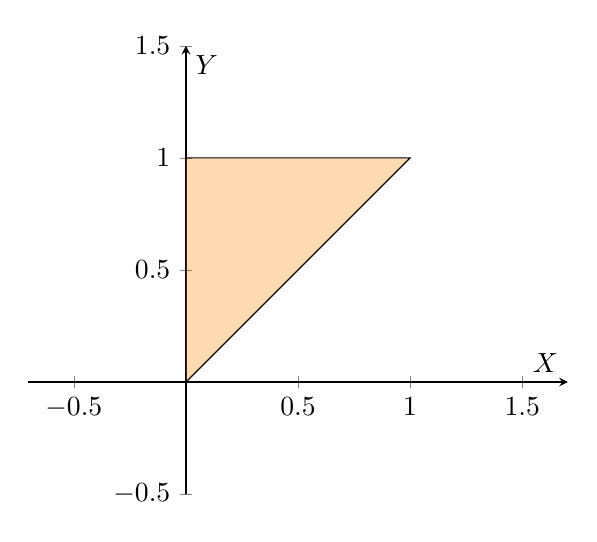
\begin{tikzpicture}
                \begin{axis}[
                    axis lines=middle,
                    xmin=-0.5, xmax=1.5,
                    ymin=-0.5, ymax=1.5,
                    xlabel={$X$},
                    ylabel={$Y$},
                    legend pos=outer north east, % Cambia la posición de la leyenda
                    axis equal,
                ]
                    
                % (0,0) (1,1) (0,1)
                \addplot[fill=orange, fill opacity=0.3] coordinates {(0,0) (1,1) (0,1)};
                \end{axis}
            \end{tikzpicture}
        \end{figure}

        Veamos ahora la función de densidad. Como se distribuye uniformemente, tenemos que:
        \begin{equation*}
            f_{(X,Y)}(x,y)=\begin{cases}
                k & (x,y)\in R_1, \\
                0 & \text{en otro caso}.
            \end{cases}
        \end{equation*}

        Para obtener el valor de $k$, tenemos que:
        \begin{align*}
            1&=\int_{0}^{1}\int_{x}^{1} k \, dy \, dx
            = k\int_{0}^{1}(1-x) \, dx
            = k\left[x-\dfrac{x^2}{2}\right]_{0}^{1}
            = k\left[1-\dfrac{1}{2}\right]
            = \dfrac{k}{2}
            \Longrightarrow k=2
        \end{align*}

        Por tanto, la función de densidad de probabilidad conjunta es:
        \begin{equation*}
            f_{(X,Y)}(x,y)=\begin{cases}
                2 & 0<x<y<1, \\
                0 & \text{en otro caso}.
            \end{cases}
        \end{equation*}

        La función generatriz de momentos conjunta es:
        \begin{align*}
            M_{(X,Y)}(t_1,t_2)&=E[e^{t_1X+t_2Y}]
            = \int_{0}^{1}\int_{x}^{1} e^{t_1x+t_2y} f_{(X,Y)}(x,y) \, dy \, dx
            =\\&= 2\int_{0}^{1}\int_{x}^{1} e^{t_1x+t_2y} \, dy \, dx
            = 2\int_{0}^{1} e^{t_1x}\int_{x}^{1} e^{t_2y} \, dy \, dx
            =\\&= 2\int_{0}^{1} e^{t_1x}\left[\dfrac{e^{t_2y}}{t_2}\right]_{x}^{1} \, dx
            = 2\int_{0}^{1} e^{t_1x}\left[\dfrac{e^{t_2}-e^{t_2x}}{t_2}\right] \, dx
            =\\&= \dfrac{2}{t_2}\int_{0}^{1} e^{t_1x+t_2}-e^{(t_1+t_2)x} \, dx
            = \dfrac{2}{t_2}\left[\dfrac{e^{t_1x+t_2}}{t_1}-\dfrac{e^{(t_1+t_2)x}}{t_1+t_2}\right]_{0}^{1}
            =\\&= \dfrac{2}{t_2}\left[\dfrac{e^{t_1+t_2}}{t_1}-\dfrac{e^{t_1+t_2}}{t_1+t_2}-\dfrac{e^{t_2}}{t_1}+\dfrac{1}{t_1+t_2}\right]
            = \dfrac{2}{t_2}\left[\dfrac{e^{t_1+t_2}-e^{t_2}}{t_1}-\dfrac{e^{t_1+t_2}-1}{t_1+t_2}\right]
        \end{align*}

        Como no podemos evaluar en el origen, sería necesario ver si la función generatriz de momentos es continua en el origen. Para ello, es necesario calcular:
        \begin{equation*}
            \lim_{(t_1,t_2)\to (0,0)} M_{(X,Y)}(t_1,t_2)
        \end{equation*}
        Este límite en varias variables es objetivo de estudio de Análisis, escapándose a los conocimientos de esta asignatura.
        \item Las distribuciones generatrices de momentos marginales.
        \item La covarianza de $X$ e $Y$.
        
        La covarianza de $X$ e $Y$ es:
        \begin{align*}
            \Cov(X,Y)&=E[XY]-E[X]E[Y]
        \end{align*}

        Calculamos cada una de las esperanzas:
        \begin{align*}
            E[X] &= \int_{0}^{1} xf_X(x) \, dx
            = \int_{0}^{1}x \int_{x}^{1} 2 \, dy \, dx
            = 2\int_{0}^{1}x(1-x) \, dx
            = 2\left[\dfrac{x^2}{2}-\dfrac{x^3}{3}\right]_{0}^{1}
            =\\&= 2\left[\dfrac{1}{2}-\dfrac{1}{3}\right]
            = \dfrac{1}{3} \\
            E[Y] &= \int_{0}^{1} yf_Y(y) \, dy
            = \int_{0}^{1}y \int_{0}^{y} 2 \, dx \, dy
            = 2\int_{0}^{1}y^2 \, dy
            = 2\left[\dfrac{y^3}{3}\right]_{0}^{1}
            = \dfrac{2}{3} \\
            E[XY] &= \int_{0}^{1}\int_{x}^{1} xyf_{(X,Y)}(x,y) \, dy \, dx
            = 2\int_{0}^{1}x \int_{x}^{1} y \, dy \, dx
            = 2\int_{0}^{1}x\left[\dfrac{y^2}{2}\right]_{x}^{1} \, dx
            =\\&= 2\int_{0}^{1}x\left[\dfrac{1}{2}-\dfrac{x^2}{2}\right] \, dx
            = 2\int_{0}^{1}\left[\dfrac{x}{2}-\dfrac{x^3}{2}\right] \, dx
            = 2\left[\dfrac{x^2}{4}-\dfrac{x^4}{8}\right]_{0}^{1}
            =\\&= 2\left[\dfrac{1}{4}-\dfrac{1}{8}\right]
            = \dfrac{1}{4}
        \end{align*}

        Por tanto, la covarianza de $X$ e $Y$ es:
        \begin{align*}
            \Cov(X,Y)&=E[XY]-E[X]E[Y]
            = \dfrac{1}{4}-\dfrac{1}{3}\cdot\dfrac{2}{3}
            = \dfrac{1}{4}-\dfrac{2}{9}
            = \dfrac{1}{36}
        \end{align*}
    \end{enumerate}
\end{ejercicio}